\documentclass[12pt,letterpaper]{article}

% ─── Packages ──────────────────────────────────────────────────────────────────
\usepackage[margin=1in]{geometry}
\usepackage{hyperref}
\usepackage{graphicx}
\usepackage{float}
\usepackage{booktabs}
\usepackage{tabularx}
\usepackage{enumitem}
\usepackage{amsmath}
\usepackage{amssymb}
\usepackage{listings}
\usepackage{xcolor}
\usepackage{tcolorbox}
\usepackage{fancyhdr}
\usepackage{titlesec}
\usepackage{caption}
\usepackage{subcaption}
\usepackage{microtype}
\usepackage{parskip}
\usepackage{tikz}
\usetikzlibrary{arrows.meta,positioning,shapes.geometric}

% ─── Code listing style ────────────────────────────────────────────────────────
\lstdefinestyle{python}{
  language=Python,
  basicstyle=\ttfamily\small,
  keywordstyle=\color{blue}\bfseries,
  commentstyle=\color{gray}\itshape,
  stringstyle=\color{orange!80!black},
  numberstyle=\tiny\color{gray},
  numbers=left,
  stepnumber=1,
  breaklines=true,
  frame=single,
  backgroundcolor=\color{gray!5},
  showstringspaces=false,
  tabsize=4,
  captionpos=b,
}

\lstdefinestyle{cpp}{
  language=C++,
  basicstyle=\ttfamily\small,
  keywordstyle=\color{blue}\bfseries,
  commentstyle=\color{gray}\itshape,
  stringstyle=\color{orange!80!black},
  numberstyle=\tiny\color{gray},
  numbers=left,
  stepnumber=1,
  breaklines=true,
  frame=single,
  backgroundcolor=\color{gray!5},
  showstringspaces=false,
}

\lstdefinestyle{bash}{
  language=bash,
  basicstyle=\ttfamily\small,
  keywordstyle=\color{teal}\bfseries,
  commentstyle=\color{gray}\itshape,
  breaklines=true,
  frame=single,
  backgroundcolor=\color{black!3},
  showstringspaces=false,
}

\lstdefinestyle{json}{
  basicstyle=\ttfamily\small,
  breaklines=true,
  frame=single,
  backgroundcolor=\color{black!3},
  showstringspaces=false,
}

% ─── Callout boxes ─────────────────────────────────────────────────────────────
\tcbuselibrary{skins,breakable}

\newtcolorbox{notebox}{
  colback=blue!5, colframe=blue!60!black,
  title=Note, fonttitle=\bfseries, breakable
}

\newtcolorbox{warningbox}{
  colback=yellow!10, colframe=orange!80!black,
  title=Warning, fonttitle=\bfseries, breakable
}

\newtcolorbox{taskbox}[1]{
  colback=green!5, colframe=green!50!black,
  title=#1, fonttitle=\bfseries, breakable
}

% ─── Header / Footer ──────────────────────────────────────────────────────────
\pagestyle{fancy}
\fancyhf{}
\rhead{Week 3: Sensor Fusion}
\lhead{MAE 162E}
\rfoot{Page \thepage}

% ─── Section formatting ────────────────────────────────────────────────────────
\titleformat{\section}{\large\bfseries}{}{0em}{\thesection\quad}
\titleformat{\subsection}{\normalsize\bfseries}{}{0em}{\thesubsection\quad}

% ─── Hyperref setup ────────────────────────────────────────────────────────────
\hypersetup{
  colorlinks=true,
  linkcolor=blue!60!black,
  urlcolor=blue!60!black,
  citecolor=green!50!black,
}

% ─── Placeholder command for diagrams ─────────────────────────────────────────
\newcommand{\diagramplaceholder}[2][4cm]{%
  \begin{center}
    \fbox{\begin{minipage}{0.85\textwidth}
      \vspace{#1}
      \centering\textit{[Diagram: #2]}
      \vspace{#1}
    \end{minipage}}
  \end{center}
}

% ═══════════════════════════════════════════════════════════════════════════════
\begin{document}
% ═══════════════════════════════════════════════════════════════════════════════

% ─── Title ────────────────────────────────────────────────────────────────────
\begin{titlepage}
  \centering
  \vspace*{2cm}
  {\Huge\bfseries MAE 162E Capstone\par}
  \vspace{0.5cm}
  {\LARGE Week 3: Sensor Fusion\par}
  \vspace{0.5cm}
  {\large Integrating IMU and ArUco-Based GPS\\for Robust Pose Estimation\par}
  \vfill
  {\small Version 1.0 \quad|\quad \today}
\end{titlepage}

\tableofcontents
\newpage

% ═══════════════════════════════════════════════════════════════════════════════
% MATERIALS LIST
% ═══════════════════════════════════════════════════════════════════════════════
\section*{Materials}
\addcontentsline{toc}{section}{Materials}

Each group will receive the following items from the course staff.
Check that all items are present before beginning the lab.

\begin{itemize}[leftmargin=2em]
  \item \textbf{ICM-20948 IMU breakout board} (SparkFun DEV-15335 or equivalent)
        --- 9 degrees of freedom: 3-axis accelerometer, 3-axis gyroscope, 3-axis
        magnetometer.
  \item \textbf{I\textsuperscript{2}C wire assembly} --- 4-conductor jumper cable
        (VCC, GND, SDA, SCL). Length: approx.\ 20~cm.
  \item \textbf{Printed ArUco tag} --- Tags are distributed by course staff;
        each group receives a \emph{unique} tag ID (IDs 11--18, 4X4\_50
        dictionary, printed at 10~cm~$\times$~10~cm).
        Do \emph{not} swap tags with another group.
        Once you receive your tag, set \texttt{TAG\_ID} at the top of
        \texttt{main.py} to match your assigned ID:
\begin{lstlisting}[style=python]
TAG_ID = 11   # replace with your group's assigned tag ID
\end{lstlisting}
\end{itemize}

% \begin{notebox}
%   The Arduino Mega 2560, Raspberry Pi~5, power board, and chassis are already
%   assembled on your robot. You only need to wire the IMU and mount your ArUco
%   tag.
% \end{notebox}

\newpage

% ═══════════════════════════════════════════════════════════════════════════════
% SECTION 1 — INTRODUCTION
% ═══════════════════════════════════════════════════════════════════════════════
\section{Introduction}

\subsection{Why Sensor Fusion?}

Every sensor carries its own kind of imperfection.
Wheel odometry integrates encoder tick counts into a position estimate: it is
smooth and responsive but \emph{drifts} --- small errors compound with every
revolution, so the estimated heading and position diverge from reality over
long runs.

Sensor fusion uses information from other sensors along with wheel odometry to produce an estimate that is
more accurate than either sensor alone.

\subsection{The Weighted-Sum (Complementary) Filter}

The simplest fusion method is the \textbf{complementary filter}, sometimes
called an \textit{alpha-blending} or \textit{weighted-sum} filter.
The idea is straightforward: at every timestep, nudge the odometry estimate a
little bit toward the absolute sensor reading.

\subsubsection*{Orientation Fusion}
An IMU measures  heading using a combination of sensing the Earth's magnetic field, using gyroscope measurements, and using accelerometer measurements:
it does not drift, but it can be \emph{noisy} and can be disturbed by nearby
motors, metal surfaces, and electrical cables.

Given:
\begin{itemize}
  \item $\theta_{\text{odom}}$ --- heading from wheel odometry (radians,
        unbounded --- accumulates past $2\pi$)
  \item $\theta_{\text{mag}}$ --- heading from the imu (radians,
        noisy)
  \item $\alpha \in [0, 1]$ --- the \emph{fusion weight} (IMU trust)
\end{itemize}

The fused heading update is:
\begin{equation}
  \hat{\theta}_{\text{fused}}
    = \theta_{\text{odom}}
    + \alpha \cdot \mathrm{wrap}\!\left(\theta_{\text{imu}} - \theta_{\text{odom}}\right)
  \label{eq:cf-heading}
\end{equation}

where $\mathrm{wrap}(\cdot)$ folds the angle difference into $[-\pi, +\pi]$
to avoid discontinuities at the $\pm 180^\circ$ boundary.

\begin{itemize}
  \item $\alpha = 0$: pure odometry --- no IMU correction.
  \item $\alpha = 1$: pure IMU --- fused heading snaps to the
        IMU reading every tick.
  \item Small $\alpha$ (e.g.\ $0.02$): gentle long-term drift correction.
        The IMU slowly pulls the estimate back toward truth without
        introducing moment-to-moment noise.
\end{itemize}

In code (\texttt{sensor\_fusion.py}):
\begin{lstlisting}[style=python, caption={ComplementaryFilter.update() in sensor\_fusion.py}]
def update(self, odom_theta, mag_heading, linear_vel, angular_vel):
    if mag_heading is None:
        return odom_theta          # no calibrated mag: fall back to odometry
    return odom_theta + self.alpha * _wrap(mag_heading - odom_theta)
\end{lstlisting}

\subsubsection*{Position Fusion}

The same idea applies to the $(x, y)$ position, replacing the IMU
with \emph{ArUco GPS} (described in Section~\ref{sec:gps-emulation}):
\begin{equation}
  \hat{\mathbf{p}}_{\text{fused}}
    = \mathbf{p}_{\text{odom}}
    + \alpha_{\text{pos}} \cdot \left(\mathbf{p}_{\text{GPS}} - \mathbf{p}_{\text{odom}}\right)
  \label{eq:cf-position}
\end{equation}

When GPS is unavailable (tag out of camera view), the robot
\emph{dead-reckons} from the last valid GPS fix using the odometry delta,
so position errors only accumulate \emph{since the last fix} rather than from
the beginning of the run.

\subsection{Other Fusion Strategies (for the Curious)}

The codebase includes two additional strategies in \texttt{sensor\_fusion.py}
that you are welcome to explore but are \emph{not} required for this lab:

\begin{itemize}
  \item \textbf{Adaptive Complementary Filter} ---
        The weight $\alpha$ decreases automatically as the robot moves faster.
        When nearly stationary the IMU is trusted more; at speed,
        odometry is more reliable short-term.

  \item \textbf{1-D Kalman Filter on Heading} ---
        A statistically optimal linear estimator. It models both
        \textit{process noise} (how much the odometry prediction can err per
        step) and \textit{measurement noise} (how noisy the IMU is).
        More principled than a fixed $\alpha$, but requires tuning two noise
        parameters instead of one.

  \item \textbf{Extended Kalman Filter (EKF)} ---
        Generalizes the Kalman filter to nonlinear systems. Standard approach
        for full 2-D/3-D pose estimation in mobile robotics; implemented in
        packages such as \texttt{robot\_localization} (ROS).
\end{itemize}

% To swap strategies in student code:
% \begin{lstlisting}[style=python, caption={Switching fusion strategy in main.py}]
% from robot.sensor_fusion import AdaptiveComplementaryFilter, HeadingKalmanFilter

% # Adaptive complementary filter (velocity-aware)
% robot.set_fusion_strategy(AdaptiveComplementaryFilter(
%     alpha_min=0.005, alpha_max=0.10))

% # Kalman filter
% robot.set_fusion_strategy(HeadingKalmanFilter(
%     process_noise=1e-4, measurement_noise=0.05))
% \end{lstlisting}

\newpage

% ═══════════════════════════════════════════════════════════════════════════════
% SECTION 2 — SYSTEM ARCHITECTURE
% ═══════════════════════════════════════════════════════════════════════════════
\section{System Architecture}

\subsection{Jetson Nano and Raspberry Pi~5 Communication}
\label{sec:jetson-rpi}

The field localization system uses a \textbf{Jetson Nano} positioned at the
side of the arena, running a RealSense D435/D455 depth camera that looks down
across the course.
Each robot's \textbf{Raspberry Pi~5} communicates with the Jetson over the
lab Wi-Fi network.

\begin{warningbox}
  The lab router performs NAT (Network Address Translation). This means
  the Jetson cannot directly initiate a connection \emph{to} the RPi. Instead,
  the \emph{RPi always initiates} the TCP connection to the Jetson on
  port~7777.  Once the socket is open, data flows in both directions and the
  NAT table entry remains alive.
\end{warningbox}

\subsubsection*{Connection Flow}

\begin{enumerate}
  \item The \texttt{robot\_gps} node starts on the RPi and opens a TCP
        connection to the Jetson at port~7777 (configurable).
  \item The Jetson accepts the connection and continuously streams
        line-delimited JSON detection messages.
  \item If the connection drops (network hiccup, container restart), the RPi
        node retries every 3~seconds automatically.
\end{enumerate}

\begin{figure}
    \centering
    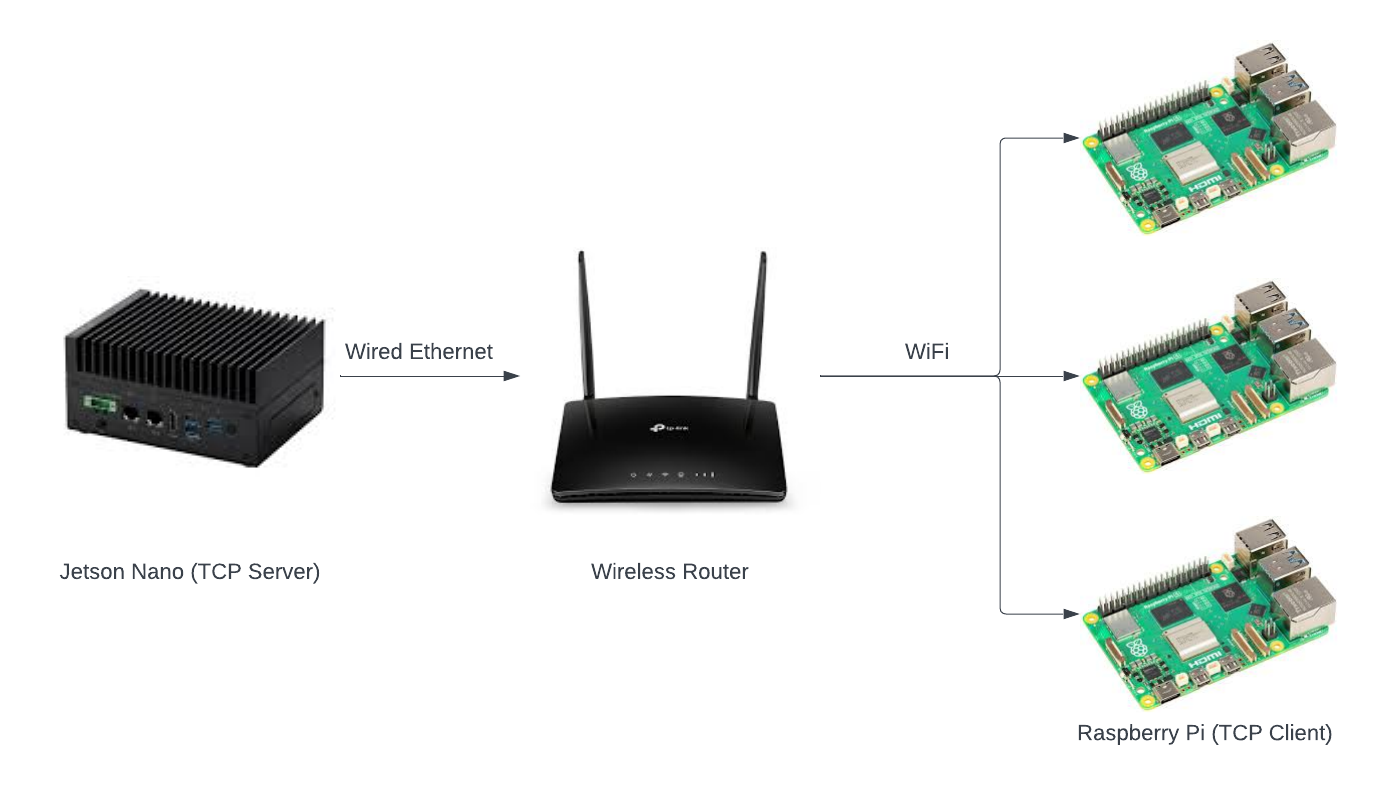
\includegraphics[width=0.8\linewidth]{figures/network_diagram.png}
    \caption{Network diagram}
    \label{fig:placeholder}
\end{figure}

\subsection{GPS Emulation via ArUco Markers}
\label{sec:gps-emulation}

Because GPS signals are unavailable indoors, we emulate global positioning
using computer vision:

\begin{itemize}
  \item \textbf{Corner anchors (IDs 0--3):} Four ArUco markers are fixed at
        the corners of the arena. The Jetson uses these to establish a
        world-frame coordinate system, with origin $(0, 0)$ at corner~0,
        $x$ pointing toward corner~1, and $y$ pointing toward corner~2.

  \item \textbf{Rover markers (IDs 11--18):} Each robot group has one unique
        marker mounted flat and visible from above.
        The Jetson detects it, projects its position onto the ground plane via
        homography, and reports $(x, y, \theta)$ in metres.
\end{itemize}

\subsubsection*{Data Format}

Detections are sent as a single line of JSON per batch:
\begin{lstlisting}[style=json, caption={GPS message format (one line per batch)}]
{"stamp": 1712345678.0,
 "detections": [{"tag_id": 11, "x": 1.23, "y": 0.45, "theta": 1.57}]}
\end{lstlisting}

The RPi converts this into a ROS~2 \texttt{TagDetectionArray} message
(metres $\to$ mm conversion happens in \texttt{robot.py}) and publishes on
\texttt{/tag\_detections}.

\subsubsection*{GPS Offset Calibration}

The Jetson's world frame origin is at the ArUco corner markers, not at
your robot's starting position.
A fixed offset maps the Jetson's world frame to the arena coordinate frame
and is already pre-measured for the venue:

\begin{lstlisting}[style=python]
# Pre-configured in test_position_fusion.py and main.py
GPS_OFFSET_X_MM = 609.6
GPS_OFFSET_Y_MM = -304.8
\end{lstlisting}

\begin{notebox}
  \textbf{You do not need to change the GPS offset.}
  These values are pre-measured for the current venue and are already set in
  both \texttt{test\_position\_fusion.py} and \texttt{main.py}.
\end{notebox}

\subsection{Venue and Coordinate System}
\label{sec:venue-coords}

The arena uses a fixed global coordinate frame established by the four corner
ArUco anchors (IDs~0--3):

\begin{itemize}
  \item \textbf{Origin $(0,\,0)$}: Corner anchor~0.
  \item \textbf{$x$-axis}: Points from corner~0 toward corner~1 (across the
        short dimension of the arena).
  \item \textbf{$y$-axis}: Points from corner~0 toward corner~2 (along the
        long dimension of the arena, toward the ramp).
\end{itemize}

The designated starting position is at the taped corner near anchor~0.
When the robot is placed correctly at the start, it should be
\textbf{pointing in the positive $y$ direction} --- that is, facing toward the
ramp.  This heading corresponds to $90^\circ$ in the standard counter-clockwise
convention (measured from the $x$-axis), which is why
\texttt{INITIAL\_THETA\_DEG = 90.0} in \texttt{main.py}.

\begin{figure}[H]
    \centering
    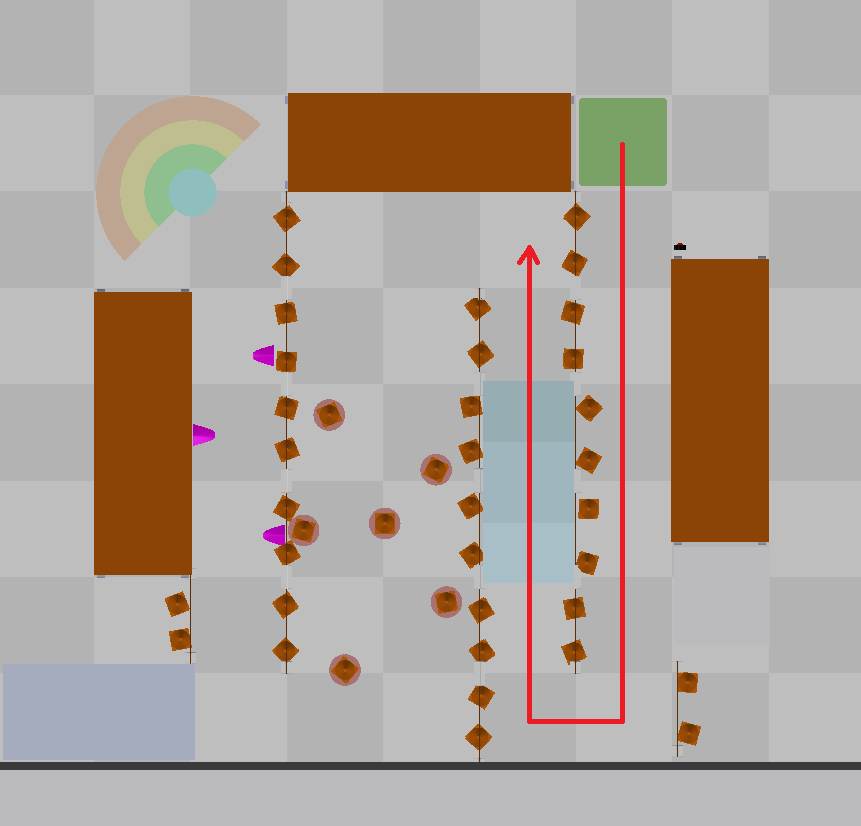
\includegraphics[width=0.5\linewidth]{figures/Venue path.png}
    \caption{Venue layout and planned path (red). The positive $y$-axis
             points toward the ramp; the robot starts pointing in this
             direction.}
    \label{fig:venue-overview}
\end{figure}

\subsection{Sensor Fusion Integration into the Existing Code}

The fusion logic is layered transparently inside the \texttt{Robot} class so
that student code in \texttt{main.py} does not need to call any fusion
functions explicitly:

\begin{enumerate}
  \item The \texttt{bridge} node publishes raw odometry on
        \texttt{/sensor\_kinematics} (25~Hz) and IMU data on
        \texttt{/sensor\_imu} (25~Hz).
  \item \texttt{robot.py} subscribes to both, plus \texttt{/tag\_detections}.
  \item On every \texttt{/sensor\_kinematics} callback, it:
    \begin{enumerate}[label=\alph*.]
      \item Incrementally unwraps the IMU heading to avoid
            $\pm 180^\circ$ discontinuities.
      \item Calls the active fusion strategy (Eq.~\ref{eq:cf-heading}).
      \item Applies the position complementary filter (Eq.~\ref{eq:cf-position}).
    \end{enumerate}
  \item \texttt{robot.get\_pose()} and \texttt{robot.get\_fused\_orientation()}
        return the fused values now.
\end{enumerate}

% \begin{notebox}
%   All sensor data is protected by a thread lock. The ROS spin thread and
%   your FSM in \texttt{main.py} run on separate threads; the \texttt{Robot}
%   API handles synchronisation transparently.
% \end{notebox}

\subsection{Changes to the Existing ROS~2 Architecture}

Table~\ref{tab:topics} summarises the topic-level changes relative to the
baseline \texttt{main} branch.

\begin{table}[H]
  \centering
  \caption{New and modified ROS~2 topics}
  \label{tab:topics}
  \begin{tabularx}{\textwidth}{llX}
    \toprule
    \textbf{Topic} & \textbf{Status} & \textbf{Description} \\
    \midrule
    \texttt{/sensor\_imu} & Pre-existing & IMU data at 25~Hz (quaternion,
        raw accel/gyro, magnetometer). Published by bridge node. \\
    \texttt{/sensor\_kinematics} & Pre-existing & Raw odometry $(x, y,
        \theta, v_x, v_y, \omega)$ at 25~Hz. \\
    \texttt{/tag\_detections} & \textbf{New} & ArUco GPS positions
        (metres, world frame). Published by \texttt{robot\_gps} node. \\
    % \texttt{/fused\_kinematics} & \textbf{New} & Fused pose
    %     $(x_{\text{fused}}, y_{\text{fused}}, \theta_{\text{fused}})$
    %     at 25~Hz. Published by robot node. \\
    \bottomrule
  \end{tabularx}
\end{table}

\begin{table}[H]
  \centering
  \caption{New and modified ROS~2 nodes}
  \label{tab:nodes}
  \begin{tabularx}{\textwidth}{llX}
    \toprule
    \textbf{Node} & \textbf{Package} & \textbf{Description} \\
    \midrule
    \texttt{robot} & \texttt{robot} & Main robot FSM; now subscribes to
        \texttt{/sensor\_imu} and \texttt{/tag\_detections}; publishes
        \texttt{/fused\_kinematics}. \\
    \texttt{robot\_gps} & \texttt{sensors} & \textbf{New.} TCP client that
        connects to Jetson and re-publishes ArUco detections as
        \texttt{TagDetectionArray}. \\
    \texttt{bridge} & \texttt{bridge} & Unchanged (UART $\leftrightarrow$
        ROS bridge). \\
    \bottomrule
  \end{tabularx}
\end{table}

\begin{figure}[H]
\centering
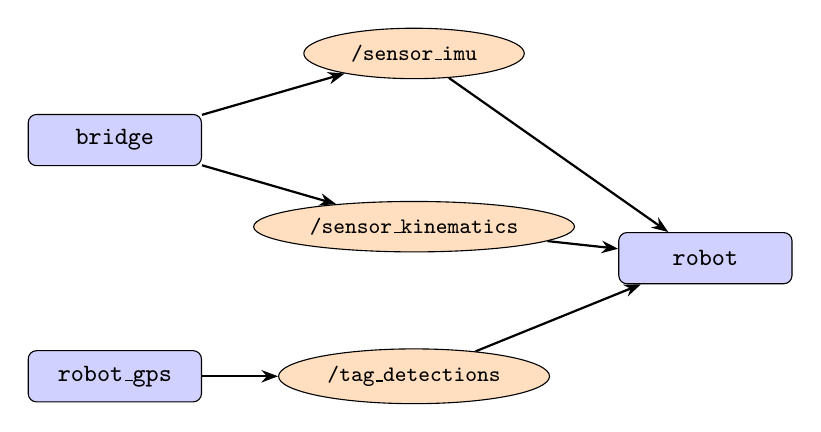
\begin{tikzpicture}[
  rosnode/.style={
    draw, rectangle, rounded corners=3pt,
    fill=blue!18, minimum width=2.2cm, minimum height=0.65cm,
    font=\ttfamily\small, text centered
  },
  rostopic/.style={
    draw, ellipse,
    fill=orange!25, minimum width=2.8cm, minimum height=0.6cm,
    font=\ttfamily\footnotesize, text centered
  },
  arr/.style={-{Stealth[length=6pt]}, thick},
]

%% ── ROS nodes ────────────────────────────────────────────────────────────────
\node[rosnode] (bridge)    at (0,    1.5)  {bridge};
\node[rosnode] (robot_gps) at (0,   -1.5)  {robot\_gps};
\node[rosnode] (robot)     at (7.5,  0)    {robot};

%% ── Topics ───────────────────────────────────────────────────────────────────
\node[rostopic] (imu)     at (3.8,  2.6)  {/sensor\_imu};
\node[rostopic] (kin)     at (3.8,  0.4)  {/sensor\_kinematics};
\node[rostopic] (tag)     at (3.8, -1.5)  {/tag\_detections};
% \node[rostopic] (fused)   at (11.0,  0)   {/fused\_kinematics};

%% ── Edges ───────────────────────────────────────────────────────────────────
\draw[arr] (bridge)    -- (imu);
\draw[arr] (bridge)    -- (kin);
\draw[arr] (imu)       -- (robot);
\draw[arr] (kin)       -- (robot);
\draw[arr] (robot_gps) -- (tag);
\draw[arr] (tag)       -- (robot);
% \draw[arr] (robot)     -- (fused)

\end{tikzpicture}

\smallskip
{\footnotesize
  \tikz\node[draw,rectangle,rounded corners=2pt,fill=blue!18,minimum width=0.9cm,minimum height=0.45cm,font=\ttfamily\tiny]{node};\;ROS\,2 node\quad
  \tikz\node[draw,ellipse,fill=orange!25,minimum width=0.9cm,minimum height=0.45cm,font=\ttfamily\tiny]{topic};\;topic
}
\caption*{\textbf{Figure:} ROS\,2 node graph for sensor fusion.}
\end{figure}

% 
\newpage

% ═══════════════════════════════════════════════════════════════════════════════
% SECTION 3 — SETUP
% ═══════════════════════════════════════════════════════════════════════════════
\section{Setup}

\subsection{List of Changed Files}

Table~\ref{tab:files} lists every file that differs between the baseline
\texttt{main} branch and the sensor-fusion branch.
Pull these changes from upstream before beginning (Section~\ref{sec:fetch}).
\begin{table}[H]
  \centering\small
  \caption{Files changed relative to baseline \texttt{main} branch}
  \label{tab:files}
  \begin{tabularx}{\textwidth}{%
    >{\ttfamily\raggedright\arraybackslash}p{0.48\textwidth}  % file path — wraps
    l                                                          % change badge
    X}                                                         % notes — fills remainder
    \toprule
    \normalfont\textbf{File} & \textbf{Change} & \textbf{Notes} \\
    \midrule
    firmware/arduino/src/config.h
      & Modified & Set \texttt{IMU\_ENABLED~1} \\[2pt]
    ros2\_ws/src/robot/robot/sensor\_fusion.py
      & \textbf{New} & ComplementaryFilter, AdaptiveComplementaryFilter,
        HeadingKalmanFilter \\[2pt]
    ros2\_ws/src/robot/robot/robot.py
      & Modified & IMU/GPS subscription callbacks, fusion logic,
        \texttt{/fused\_kinematics} publisher \\[2pt]
    ros2\_ws/src/robot/robot/main.py
      & Modified & Pure-pursuit path planner integration, student task
        scaffolding \\[2pt]
    ros2\_ws/src/robot/robot/\\test\_orientation\_fusion.py
      & \textbf{New} & Orientation fusion test harness \\[2pt]
    ros2\_ws/src/robot/robot/\\test\_position\_fusion.py
      & \textbf{New} & Position fusion test harness \\[2pt]
    ros2\_ws/src/robot/launch/\\test\_orientation\_fusion.launch.py
      & \textbf{New} & Launch file for orientation test \\[2pt]
    ros2\_ws/src/robot/launch/\\test\_position\_fusion.launch.py
      & \textbf{New} & Launch file for position test \\[2pt]
    ros2\_ws/src/sensors/sensors/\\robot\_gps\_node.py
      & \textbf{New} & TCP bridge to Jetson ArUco detector \\[2pt]
    ros2\_ws/src/robot/launch/robot.launch.py
      & Modified & Adds \texttt{robot\_gps} node to launch graph \\
    \bottomrule
  \end{tabularx}
\end{table}

\subsection{Fetching from Upstream/Main}
\label{sec:fetch}

Run the following commands to pull the
latest changes:

\begin{lstlisting}[style=bash, caption={Fetching and building the sensor fusion branch}]
# Inside the Project-NUEVO/ directory

# Pull latest changes from the main branch
git fetch upstream
git rebase upstream/main

\end{lstlisting}

\begin{notebox}
  If you have local changes in \texttt{main.py}, Git may report a merge
  conflict. Resolve conflicts manually in your editor, then run
  \texttt{git add} and \texttt{git merge --continue}.
\end{notebox}

\subsection{Enabling the IMU in the Arduino Firmware}

By default, the IMU is disabled in the firmware to save boot time on robots
that have no sensor attached.
You must enable it, recompile, and re-upload.

\begin{enumerate}
  \item Open \texttt{firmware/arduino/src/config.h} and find the line:
\begin{lstlisting}[style=cpp]
#define IMU_ENABLED   0
\end{lstlisting}
        Change it to:
\begin{lstlisting}[style=cpp]
#define IMU_ENABLED   1
\end{lstlisting}

  \item Recompile and upload according to Week 1 instructions for flashing Arduino firmware

  \item Verify: the bridge log should print IMU telemetry lines at 25~Hz
        once the firmware enters \texttt{RUNNING} state.
\end{enumerate}

\subsection{Connecting the IMU}

The ICM-20948 communicates over the I\textsuperscript{2}C bus.
Connect the breakout board to the Arduino Mega using the provided
I\textsuperscript{2}C wire assembly.

\begin{warningbox}
  Power down the robot completely before making or changing any wiring
  connections. Connecting the IMU to a live board can damage both the
  Arduino and the sensor.
\end{warningbox}

% \begin{table}[H]
%   \centering
%   \caption{IMU wiring to Arduino Mega 2560}
%   \label{tab:wiring}
%   \begin{tabular}{lll}
%     \toprule
%     \textbf{IMU Pin} & \textbf{Arduino Pin} & \textbf{Notes} \\
%     \midrule
%     VCC & 3.3V & Do \emph{not} connect to 5~V --- sensor is 3.3~V logic \\
%     GND & GND & Any GND pin \\
%     SDA & Pin 20 (SDA) & Hardware I\textsuperscript{2}C bus \\
%     SCL & Pin 21 (SCL) & Hardware I\textsuperscript{2}C bus \\
%     AD0 & 3.3V & Sets I\textsuperscript{2}C address to 0x69 \\
%     \bottomrule
%   \end{tabular}
% \end{table}

% \diagramplaceholder[4cm]{IMU wiring diagram: SparkFun ICM-20948 breakout $\to$ Arduino Mega 2560. Show 4-wire connection with colour coding (red=VCC, black=GND, blue=SDA, yellow=SCL) and the AD0 pull-up.}

% \begin{notebox}
%   The SparkFun ICM-20948 breakout has AD0 high by default (connected
%   internally to 3.3~V via a pull-up resistor), giving I\textsuperscript{2}C
%   address \texttt{0x69}.  This matches \texttt{IMU\_AD0\_VAL~1} in
%   \texttt{config.h} --- no change needed.
% \end{notebox}

\subsection{Mounting the ArUco Tag}

\begin{enumerate}
  \item Attach your printed ArUco tag to the top flat surface of the robot
        so it is clearly visible from directly above.
  \item Keep the tag level with respect to the floor --- tilt causes measurement error.
  \item \textbf{Align the tag with the robot axes:} mount the tag so that
        the sides of the printed square are parallel to the robot's forward
        and sideways axes.  Rotation of the tag relative to the robot body
        introduces a systematic heading error in the camera-derived pose.
  \item \textbf{Center the tag on the drive-axle line:} the localization
        system reports the tag's position in the world frame; it then
        subtracts a body-frame offset to recover the robot's wheel-center
        position.  If your tag is not directly above the midpoint of the
        line connecting the two drive wheels, measure the offset and set
        the following constants in \texttt{robot.py}:
\begin{lstlisting}[style=python, caption={Tag body-frame offset in robot.py}]
TAG_X_OFFSET_MM = 0.0  # forward offset of tag from wheel-axle centre (mm)
TAG_Y_OFFSET_MM = 0.0  # sideways offset of tag from wheel-axle centre (mm)
\end{lstlisting}
        Positive $x$ is forward, positive $y$ is to the left.
        If the tag is centred on the axle midpoint (recommended), leave
        both values at \texttt{0.0}.
  \item Make sure the tag ID matches the one assigned to your group
        (printed on the tag envelope).
\end{enumerate}

\begin{figure}
    \centering
    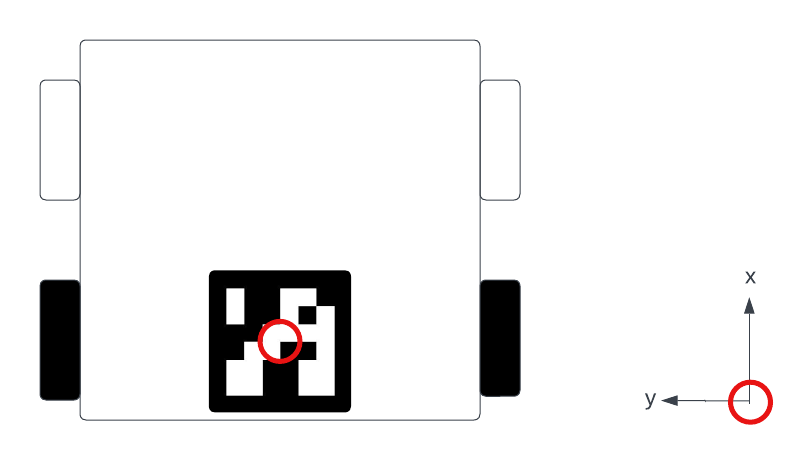
\includegraphics[width=0.5\linewidth]{figures/arucotag_mounting.png}
    \caption{ArUco tag mounting}
    \label{fig:aruco-mounting}
\end{figure}

\subsection{IMU Calibration}

The IMU must be calibrated before any fusion test will work
correctly.

\begin{enumerate}
  \item Start the Docker stack and bring the bridge up:
\begin{lstlisting}[style=bash]
docker compose -f ros2_ws/docker/docker-compose.rpi.yml up -d
docker compose exec ros2_runtime bash
ros2 run bridge bridge
\end{lstlisting}
  \item In the NUEVO front end UI, you should see the IMU show up. Calibration can be performed from there.
\end{enumerate}

% \begin{notebox}
%   Perform calibration on the actual arena surface, away from large metal
%   objects and power cables.  Moving the robot to a different location after
%   calibration may change the ambient field slightly, but the saved offsets
%   are a good starting point.
% \end{notebox}

\newpage

% ═══════════════════════════════════════════════════════════════════════════════
% SECTION 4 — TASKS
% ═══════════════════════════════════════════════════════════════════════════════
\section{Tasks}

% ──────────────────────────────────────────────────────────────────────────────


\subsection{Task 1: Sensor Fusion Tuning}

\begin{taskbox}{Task 1 Overview}
  Drive the robot through preprogrammed manoeuvres while varying the
  fusion weight $\alpha$.  Observe how $\alpha$ affects the trade-off between
  odometry smoothness and absolute accuracy, then choose a good value to carry
  forward into Task~2.
\end{taskbox}

% ─── Sub-task 1a ──────────────────────────────────────────────────────────────
\subsubsection{Sub-task 1a: Orientation Fusion}

\textbf{Setup:} Take the robot to an open area of the lab floor.

\textbf{Procedure:}
\begin{enumerate}
  \item Start the Docker stack and, in one terminal inside the container,
        start the bridge:
\begin{lstlisting}[style=bash]
docker compose -f ros2_ws/docker/docker-compose.rpi.yml up -d
docker compose exec ros2_runtime bash
ros2 run bridge bridge
\end{lstlisting}
  \item Open \texttt{ros2\_ws/src/robot/robot/test\_orientation\_fusion.py}
        and set the fusion weight (FUSION\_ALPHA) at the top of the file:
\begin{lstlisting}[style=python, caption={Tunable parameters in test\_orientation\_fusion.py}]
CIRCLE_RADIUS_MM  = 300.0   # mm
DRIVE_SPEED_MM_S  = 100.0   # mm/s
NUM_LAPS          = 2
FUSION_ALPHA      = 0.02    # <-- edit this value (0.0 to 1.0)
\end{lstlisting}
  \item In a \textbf{second terminal} inside the container, launch the test:
\begin{lstlisting}[style=bash]
docker compose exec ros2_runtime bash
ros2 launch robot test_orientation_fusion.launch.py
\end{lstlisting}
        The robot will drive two circles of radius 300~mm at 100~mm/s
        (approximately 19~seconds per lap).
  \item After the test finishes, copy the result image to the host and view
        it in VS~Code.  Run the following \textbf{outside Docker} in a
        VS~Code terminal:
\begin{lstlisting}[style=bash]
docker cp docker-ros2_runtime-1:/root/orientation_fusion_test_result.png \
    ~/Project-NUEVO/
\end{lstlisting}
        Then navigate to \texttt{\textasciitilde/Project-NUEVO} in the
        VS~Code file explorer and \textbf{Ctrl-click} the image file to
        open it.
  \item The plot has three panels:
        \begin{itemize}
          \item \textbf{Panel 1:} Robot trajectory coloured by the magnitude of
                the fusion correction $|\hat\theta_{\text{fused}} - \theta_{\text{odom}}|$.
          \item \textbf{Panel 2:} Odometry heading vs.\ fused heading over
                time.
          \item \textbf{Panel 3:} Per-sample fusion correction
                $\hat\theta_{\text{fused}} - \theta_{\text{odom}}$ over time.
        \end{itemize}
  \item Repeat with at least three different values of \texttt{FUSION\_ALPHA}
        (e.g.\ $0.0$, $0.02$, $0.5$, $1.0$).
\end{enumerate}

% \textbf{Questions to explore:}
% \begin{itemize}
%   \item At $\alpha = 0$, do the two heading traces match?
%         What does this tell you?
%   \item At $\alpha = 1$, how noisy does the fused heading become?
%   \item At what value of $\alpha$ does the fused heading stay smooth while
%         still correcting the odometry drift after two laps?
%   \item Is the correction larger at the beginning or end of each lap?  Why?
% \end{itemize}

\begin{notebox}
  Record the $\alpha$ value you choose that gives you the best results. You will need it in Task~2 when you
  configure \texttt{main.py}.
\end{notebox}

\begin{warningbox}
  \textbf{Orientation fusion is disabled in the actual robot run
  (\texttt{ORIENTATION\_ALPHA = 0.0} in \texttt{robot.py}).}
  The IMU magnetometer does not operate accurately in the presence of the
  strong magnetic fields produced by the motors and nearby metal surfaces in
  the current lab.  Setting \texttt{ORIENTATION\_ALPHA = 0} means the robot
  relies on pure wheel odometry for heading, avoiding IMU-induced errors.
  Task~1a is a learning exercise to understand the complementary filter
  trade-offs; you should \emph{not} set \texttt{ORIENTATION\_ALPHA > 0} in
  \texttt{main.py} for the actual course run.
\end{warningbox}

\begin{notebox}
  \textbf{IMU mounting orientation (\texttt{IMU\_Z\_DOWN} in
  \texttt{robot.py}):} If the IMU board is mounted with its $z$-axis pointing
  downward (chip face down), set \texttt{IMU\_Z\_DOWN = True} so the yaw sign
  is corrected in software.  In our current setup the chip faces upward, so
  the default \texttt{IMU\_Z\_DOWN = False} is correct.  This parameter is
  academic given that orientation fusion is disabled, but you are welcome to
  experiment with it.
\end{notebox}

% ─── Sub-task 1b ──────────────────────────────────────────────────────────────
\subsubsection{Sub-task 1b: Position Fusion}

\textbf{Setup:}
\begin{enumerate}
  \item Place the robot at the designated starting position
        (marked by tape on the arena floor, along the ramp approach).
        The starting corner of the robot chassis should align with the tape
        marks.  The robot must be \textbf{facing the positive $y$ direction}
        (toward the ramp) --- see Section~\ref{sec:venue-coords} for the
        coordinate system.
  \item Ensure the Jetson Nano is running and its camera can see your ArUco
        tag from above.
\end{enumerate}

\textbf{Tunable Parameter:}

The GPS fusion weight \texttt{POSITION\_ALPHA} controls how aggressively the
fused position is pulled toward the GPS reading each timestep.
It is defined as a class constant in \texttt{robot.py}:
\begin{lstlisting}[style=python, caption={POSITION\_ALPHA in robot.py}]
POSITION_ALPHA = 0.10  # GPS weight for position fusion (0.0 to 1.0)
\end{lstlisting}
Increase this value to trust GPS more; decrease it to rely more on odometry.
You will tune this by observing how the robot tracks the straight-line path
during the test.

\textbf{Procedure:}
\begin{enumerate}
  \item If not already running, start the bridge in one terminal inside the
        container:
\begin{lstlisting}[style=bash]
docker compose -f ros2_ws/docker/docker-compose.rpi.yml up -d
docker compose exec ros2_runtime bash
ros2 run bridge bridge
\end{lstlisting}
  \item In a \textbf{second terminal} inside the container, launch the test:
\begin{lstlisting}[style=bash]
docker compose exec ros2_runtime bash
ros2 launch robot test_position_fusion.launch.py
\end{lstlisting}
        The robot drives straight forward for 1000~mm.
  \item The result plot is saved directly to \texttt{\textasciitilde/Project-NUEVO/}
        on the host --- no \texttt{docker cp} needed.
        In a VS~Code terminal navigate to \texttt{\textasciitilde/Project-NUEVO}
        and \textbf{Ctrl-click}
        \texttt{position\_fusion\_test\_result.png} to open it.
        The plot shows four panels: X over time, Y over time, 2-D trajectory,
        and position error magnitude (GPS-active periods shaded green).
  \item Repeat with \texttt{POSITION\_ALPHA} = $0.0$, $0.5$, $1.0$ (edit the
        value in \texttt{robot.py} and relaunch each time).
        Also try temporarily removing your tag for a
        few seconds mid-run to observe dead-reckoning behaviour.
\end{enumerate}

% \textbf{Questions to explore:}
% \begin{itemize}
%   \item During GPS-active periods, how does the fused path differ from
%         the raw odometry path?
%   \item When you block the tag, what happens to the fused position?
%         Does it freeze, jump, or follow odometry?
%   \item What happens to position error right after GPS comes back online?
%   \item Why is $\alpha = 1.0$ (snap entirely to GPS each tick) probably
%         \emph{not} a good choice, even though GPS is more accurate?
% \end{itemize}

% ──────────────────────────────────────────────────────────────────────────────
\subsection{Task 2: Obstacle Course Navigation}

\begin{taskbox}{Task 2 Overview}
  Modify \texttt{main.py} to give the robot a set of waypoints that navigate
  through the full obstacle course. The robot must use the fused pose
  (heading $+$ position) from Task~1 to stay on path.
\end{taskbox}

\subsubsection{Course Description}

The course is set up on the arena floor (see Figure~\ref{fig:venue-overview}
in Section~\ref{sec:venue-coords}). Key features:
\begin{itemize}
  \item \textbf{Start:} Predefined corner, robot placed against tape markers.
  \item \textbf{Ramp:} The robot must drive over the ramp (note: position sensor fusion is useful here)
  \item \textbf{Finish:} End within the tile boundaries
\end{itemize}

\subsubsection{Modifying \texttt{main.py}}

Open \texttt{ros2\_ws/src/robot/robot/main.py}.

\begin{notebox}
  \textbf{Starting heading (\texttt{INITIAL\_THETA\_DEG}):}
  The top of \texttt{main.py} sets
\begin{lstlisting}[style=python]
INITIAL_THETA_DEG = 90.0
\end{lstlisting}
  This tells the odometry system that the robot starts pointing at $90^\circ$,
  which corresponds to the positive $y$ direction in the arena frame (toward
  the ramp) --- see Section~\ref{sec:venue-coords}.
  \textbf{You do not need to change this value} provided you place the robot at
  the taped starting position with the robot pointing forward (toward the ramp).
\end{notebox}

In the \texttt{INIT} block, replace the placeholder waypoints with the course waypoints.
All coordinates are in \textbf{millimetres}, in the arena frame
(origin at start corner, $x$ across, $y$ toward the ramp).

\begin{lstlisting}[style=python, caption={Obstacle course waypoints in main.py (fill in from the course diagram)}]
path_control_points = [
    # (x_mm, y_mm)
    (   0.0,     0.0),   # Start
    (   0.0,   ???.?),   # Waypoint 1 -- fill in from diagram
    ( ???.0,   ???.0),   # Waypoint 2
    # ... add remaining waypoints ...
    (   0.0,     0.0),   # Return to start
]
\end{lstlisting}

\begin{notebox}
  Use the \texttt{POSITION\_ALPHA} value you found in Task~1b.
  Edit the constant directly in \texttt{robot.py} before launching, or
  override it at runtime via \texttt{robot.set\_pos\_fusion\_alpha()} at the
  top of \texttt{run()} in \texttt{main.py}:
\begin{lstlisting}[style=python]
def run(robot: Robot) -> None:
    configure_robot(robot)
    # ORIENTATION_ALPHA stays 0.0 (set in robot.py) -- do not override
    robot.set_pos_fusion_alpha(0.10)   # position fusion weight from Task 1b
    # ... rest of run() ...
\end{lstlisting}
\end{notebox}

\subsubsection{Completing the MOVING State}

The \texttt{MOVING} state in \texttt{main.py} contains step-by-step
scaffolding (Steps 1--8) that you must implement.
The core loop reads the fused pose, advances the path, computes a lookahead
point, calculates velocity commands, and checks for goal arrival.

\begin{lstlisting}[style=python, caption={MOVING state skeleton in main.py (complete Steps 1--8)}]
elif state == "MOVING":
    show_moving_leds(robot)

    # Step 1: Read fused pose
    current_x, current_y, current_theta_deg = robot.get_pose()

    # Step 2: Convert heading to radians
    current_theta_rad = math.radians(current_theta_deg)

    # Step 3: Advance the remaining path
    remaining_path = planner1._advance_remaining_path(
        remaining_path, current_x, current_y, advance_radius=20.0)

    # Step 4: Compute lookahead point
    current_pursuit_x, current_pursuit_y = \
        planner1._lookahead_point(
            remaining_path, current_x, current_y, current_theta_rad)

    # Step 5: Compute velocity command
    lin_vel, ang_vel = planner1.compute_velocity(
        current_x, current_y, current_theta_rad,
        current_pursuit_x, current_pursuit_y)

    # Step 6: Send velocity command
    robot.set_velocity(lin_vel, math.degrees(ang_vel))

    # Step 7: Check goal reached
    if planner1.CurrentTargetReached(
            current_pursuit_x, current_pursuit_y,
            current_x, current_y):
        robot.stop()
        state = "IDLE"
\end{lstlisting}

\subsubsection{Running the Course}

\begin{enumerate}
  \item Place the robot at the taped start position.
  \item In one terminal inside the Docker container, start the bridge:
\begin{lstlisting}[style=bash]
docker compose -f ros2_ws/docker/docker-compose.rpi.yml up -d
docker compose exec ros2_runtime bash
ros2 run bridge bridge
\end{lstlisting}
  \item In a \textbf{second terminal} inside the container, launch the full
        robot stack:
\begin{lstlisting}[style=bash]
docker compose exec ros2_runtime bash
ros2 launch robot robot.launch.py
\end{lstlisting}
  \item Verify that the bridge is connected and the firmware is in
        \texttt{IDLE} state (orange LED on).
  \item Press \textbf{BTN\_1} on the robot to enter \texttt{MOVING} state
        (green LED on).
  \item Monitor the console output for pose and pursuit-point debug prints.
  \item If the robot deviates significantly, stop it with Ctrl-C, adjust
        waypoints or fusion weights, and relaunch.
  \item After the run, copy the trajectory plot to the host and view it in
        VS~Code.  Run the following \textbf{outside Docker} in a VS~Code
        terminal:
\begin{lstlisting}[style=bash]
docker cp docker-ros2_runtime-1:/ros2_ws/trajectory.png ~/Project-NUEVO/
\end{lstlisting}
        Then navigate to \texttt{\textasciitilde/Project-NUEVO} in the
        VS~Code file explorer and \textbf{Ctrl-click} \texttt{trajectory.png}
        to open it.
\end{enumerate}

\newpage

% ═══════════════════════════════════════════════════════════════════════════════
% SECTION 5 — DELIVERABLE
% ═══════════════════════════════════════════════════════════════════════════════
\section{Deliverable}

\begin{taskbox}{Lab Deliverable}
  Demonstrate your robot completing the full obstacle course \emph{without
  any manual intervention} (no pushing, nudging, or repositioning once
  \texttt{BTN\_1} is pressed).
\end{taskbox}

The demonstration must satisfy all of the following criteria:

\begin{enumerate}
  \item The robot starts from the designated starting position.
  \item It navigates over the ramp.
  \item It passes through all designated waypoints in order.
  \item It finishes within the tile boundaries.
  \item Sensor fusion (both orientation and position) must be active
        (i.e.\ \texttt{FUSION\_ALPHA~>~0} and \texttt{POS\_FUSION\_ALPHA~>~0}).
\end{enumerate}

% \textbf{Grading Notes:}
% \begin{itemize}
%   \item A run that completes the course with the robot touching a pylon
%         (but not knocking it over) will receive partial credit.
%   \item You may run the course as many times as needed during the demo
%         period.
%   \item Be prepared to show the console output and explain your choice
%         of $\alpha$ values.
% \end{itemize}

\newpage

% ═══════════════════════════════════════════════════════════════════════════════
% APPENDIX
% ═══════════════════════════════════════════════════════════════════════════════
\appendix
\section{Quick-Reference: Robot API Methods Used in This Lab}

\begin{tabularx}{\textwidth}{lX}
  \toprule
  \textbf{Method} & \textbf{Description} \\
  \midrule
  \texttt{robot.get\_pose()} &
    Returns \texttt{(x, y, theta\_deg)} in the configured unit (mm by
    default). Uses fused position and odometry heading.\\[4pt]
  \texttt{robot.get\_fused\_orientation()} &
    Returns the fused heading in degrees (IMU-corrected). \\[4pt]
  \texttt{robot.set\_velocity(lin, ang\_deg\_s)} &
    Commands linear velocity (mm/s) and angular velocity (deg/s). \\[4pt]
  \texttt{robot.stop()} &
    Sends a zero-velocity command immediately. \\[4pt]
  \texttt{robot.set\_fusion\_alpha(alpha)} &
    Sets the heading complementary-filter weight (0--1). \\[4pt]
  \texttt{robot.set\_pos\_fusion\_alpha(alpha)} &
    Sets the position complementary-filter weight (0--1). \\[4pt]
  \texttt{robot.set\_gps\_offset(x\_mm, y\_mm)} &
    Sets the GPS world-frame to arena-frame offset. \\[4pt]
  \texttt{robot.is\_gps\_active()} &
    Returns \texttt{True} if a GPS fix was received within the last 1~s. \\[4pt]
  \texttt{robot.reset\_odometry()} &
    Resets the firmware odometry to the initial heading. \\
  \bottomrule
\end{tabularx}

\section{Troubleshooting}

\begin{tabularx}{\textwidth}{lX}
  \toprule
  \textbf{Symptom} & \textbf{Fix} \\
  \midrule
  IMU data not appearing in bridge log &
    Check \texttt{IMU\_ENABLED 1} in \texttt{config.h} and re-upload.
    Verify SDA/SCL wiring with a multimeter. \\[4pt]
  \texttt{/tag\_detections} topic empty &
    Ensure \texttt{robot\_gps} node is running. Check that the Jetson
    Docker container is up and the tag is visible to the camera. \\[4pt]
  IMU magnetometer always shows \texttt{calibrated: false} &
    Redo calibration. \\[4pt]
  Robot spins in place or drives erratically &
    Check that \texttt{LEFT\_WHEEL\_DIR\_INVERTED} and
    \texttt{RIGHT\_WHEEL\_DIR\_INVERTED} match your physical wiring.
    Run \texttt{ros2 echo /sensor\_kinematics} to inspect odometry. \\[4pt]
  GPS position jumps discontinuously &
    Set \texttt{POS\_FUSION\_ALPHA} to a smaller value (e.g.\ 0.3) so GPS
    corrections are applied gradually. \\[4pt]
  Fused heading drifts even with IMU active &
    Increase \texttt{FUSION\_ALPHA} slightly. Verify calibration was
    performed on the arena. \\
  \bottomrule
\end{tabularx}

\end{document}
